\chapter{Estructura estelar}
\REMARK{The Development of the Theory of Stellar Structure}
\TODO{Breve introducción al capítulo más teórico de la tesis. Por qué es importante el estudio de la estructura estelar en equilibrio tanto en el caso newtoniano como en el relativista. Algo de historia de quienes desarrollaron lo que presento en el caso relativista y las condiciones de aceptabilidad física que se han establecido para discernir entre modelos. }

\section{Caso newtoniano}\TODO{Basado en los comentarios de la propuesta modificar esta sección}

Considerando una distribución de materia con simetría esférica, si $r$ denota la distancia desde el centro de la configuración, la masa encerrada en una superficie esférica de radio $r$ será:  
\begin{equation}
    m ( r ) = \int _ { 0 } ^ { r } 4 \pi r ^ { 2 } \rho \dd{r} = \int_{0}^{r} \dd{m(r)} \quad\text{con}\quad \dd{m(r)}=4\pi r^2\rho \dd{r},
    \label{mN}
\end{equation}

\begin{equation}
    \Longrightarrow\dv{m(r)}{r} =4\pi r^2 \rho.
    \label{dmnewton}
\end{equation}
Ahora, se considera un cilindro infinitesimal a una distancia $r$ del centro, de altura $\dd{r}$ y sección transversal unitaria, normal al vector posición $\vec{r}$ (ver Figura \ref{stellnew}).  

\begin{figure}[H]
    \centering
    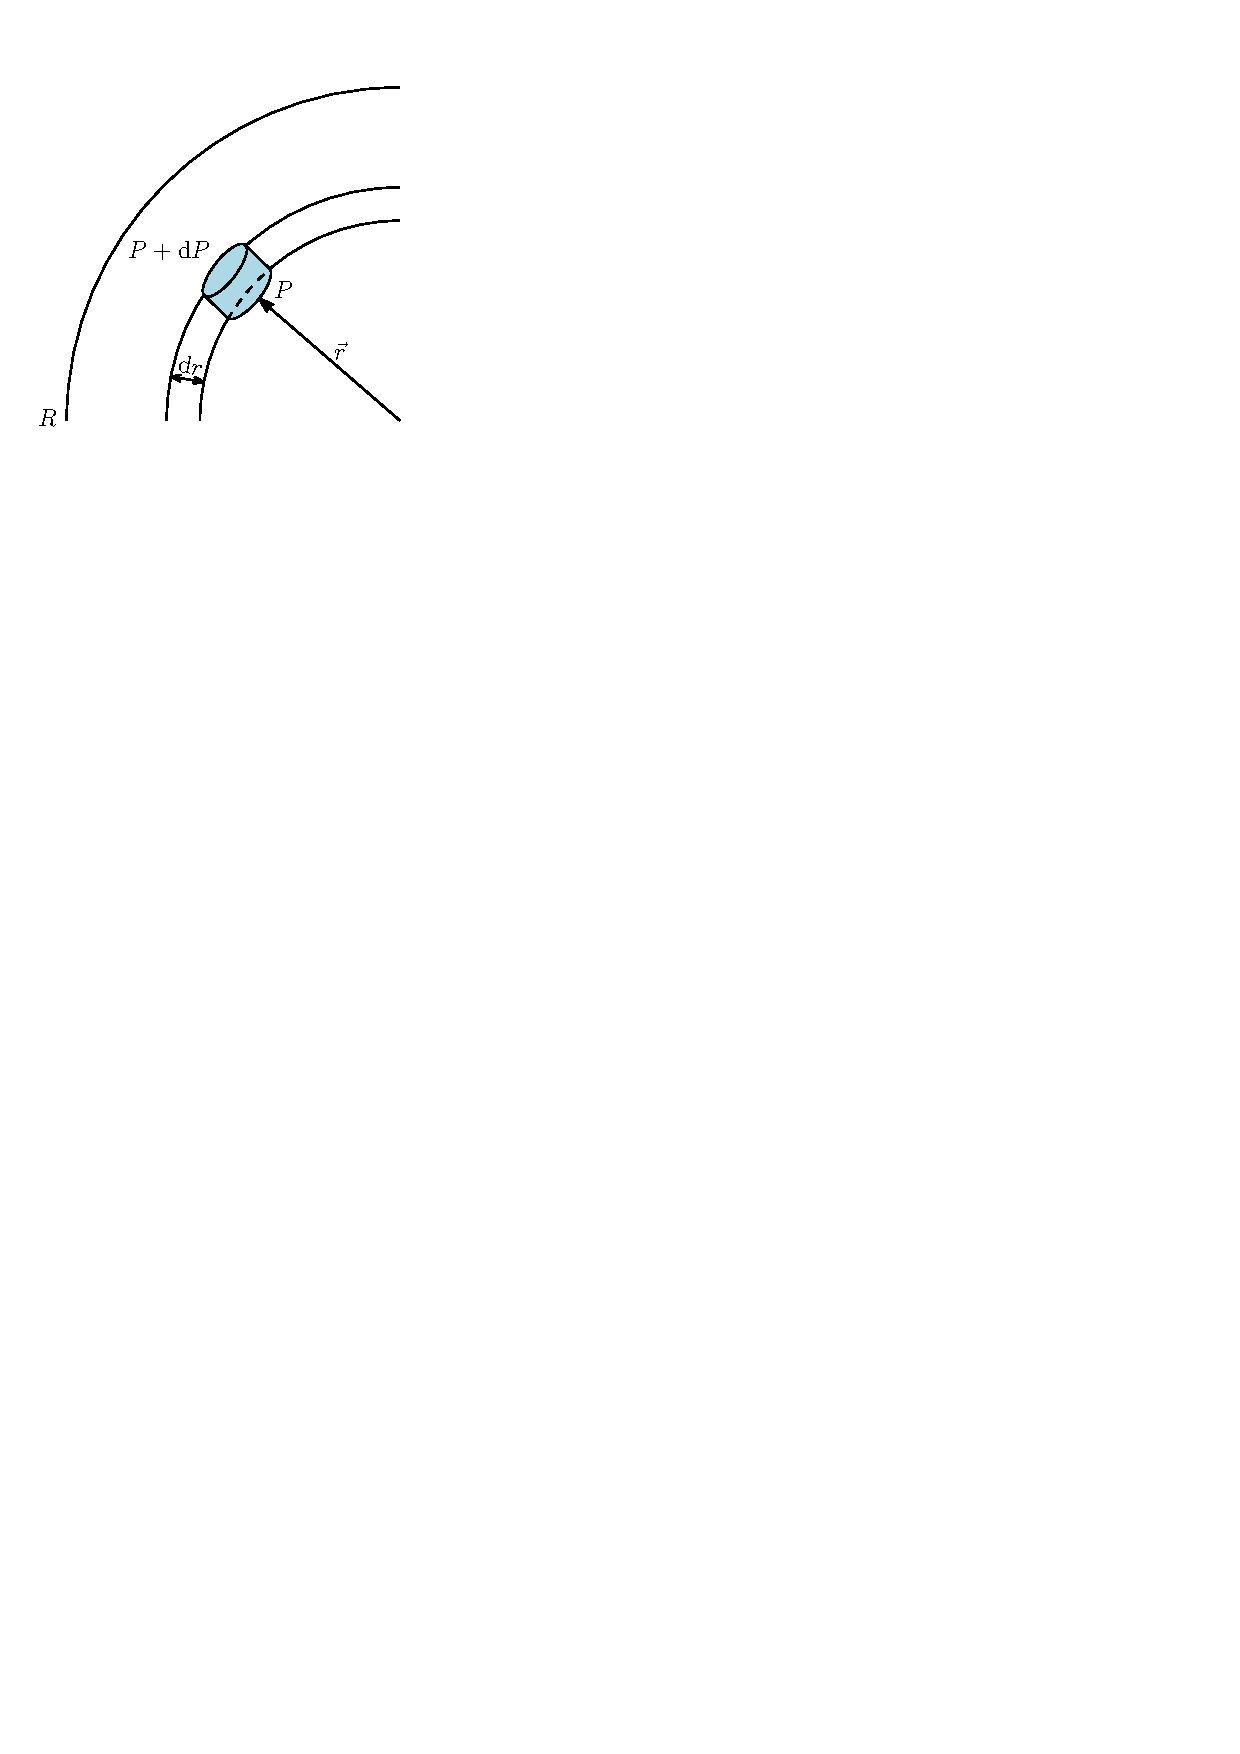
\includegraphics[width=150pt]{figures/stellarnewton.pdf}
    \caption{Presión sobre un elemento de masa cilíndrico.}
    \label{stellnew}
\end{figure}
Si la presión en $\vec{r}$ es $P$ y su cambio al ir de $\vec{r}$ a $\vec{r}+\dd{\vec{r}}$ es $\dd{P}$. Suponiendo que el elemento de área es $dA$ la diferencia de presión representa una fuerza 
\begin{equation*}
    F_{Pelem}=-\dd{P}\dd{A},
\end{equation*}
actuando sobre el elemento de masa. Esta fuerza debe contrarrestar la atracción gravitacional sobre el elemento de masa debido a $m(r)$
\begin{equation*}
    F_{atracc}=\frac{G m(r)\rho \dd{A} \dd{r}}{r^2}.
\end{equation*}
Para que el elemento de masa se encuentre en equilibrio se requiere entonces:

\begin{equation}
    -\dd{P}\dd{A} =\frac{G m(r)\rho \dd{A} \dd{r}}{r^2},
\end{equation}
o
\begin{equation}
    \dv{P}{r} = - \frac { G m ( r ) } { r ^ { 2 } } \rho.
    \label{dpnewton}
\end{equation}
que es la conocida ecuación de equilibrio hidrostático. 

Las ecuaciones \eqref{dmnewton} y \eqref{dpnewton} son las ecuaciones de estructura estelar newtonianas \cite{Chandrasekhar1958}. Si una relación entre la presión y la densidad $P(\rho)$ es dada, es decir, una ecuación de estado, el sistema puede resolverse dado un par condiciones iniciales $m(r=0)$ y $P(r=0)$. La primera de estas condiciones es evidente puesto que no hay masa encerrada en un cascarón esférico de radio nulo, $m(r=0)=0$. La segunda estará definida por el valor de $\rho(r=0)\equiv\rho_c$ escogido, mediante la ecuación de estado, $P(r=0)=P(\rho_c)$.

El radio de la estrella $R$ se define como el valor de $r$ en el que la presión se anula, esto es, $P(R)=0$ y de manera similar la masa de la estrella $M$ se define como el valor de la masa encerrada en $r=R$, esto es, $m(R)=M$.

\REMARK{Decidir si mantener o no} Aunque no se van a tratar en este trabajo, cabe resaltar que las \emph{enanas blancas} son bien descritas por las ecuaciones de estructura newtonianas. Una manera, aunque no la única, de conocer la importancia de las correcciones relativistas es comparando el valor de $\frac{2GM}{c^2R}$ con la unidad (la razón será evidente en el resultado relativista) \cite{Weinberg1972}. Las enanas blancas tienen masas en un rango de $0.33\,M_{\odot}$ $1.52\,M_{\odot}$ y radios típicos de unos cuantos miles de kilómetros \cite{Glendenning2000}. Para una enana blanca promedio, con masa $M=0.6\,M_{\odot}$ y radio $r=3000 \,\rm{km}$ se tiene
\begin{equation}
    \frac{2GM}{c^2R}\simeq 6\times 10^{-4}\ll 1,
\end{equation}
por lo cual se espera que el tratamiento newtoniano sea suficiente. 

\section{Caso relativista}\label{CR}\TODO{Basado en los comentarios de la propuesta modificar esta sección. Teniendo en cuenta que los cálculos están hechos en el apéndice.}

%Si bien en la teoría newtoniana podrían existir objetos tan compactos como las estrellas de neutrones, algunas de las predicciones presentan inconsistencias con lo predicho por la teoría de la Relatividad General. Por ejemplo, Chandrasekhar encontró (usando gravedad newtoniana) que las estrellas soportadas por presión de degeneración tienen una masa máxima, obtenida asintóticamente cuando los fermiones son altamente relativistas. Esto es, cuando tienen velocidades comparables con la velocidad de la luz. Bajo tales condiciones la teoría newtoniana permitiría la existencia de estrellas compuestas por los quarks más pesados (charm, bottom y top). En Relatividad General se predice también la existencia de una masa máxima, pero ésta no es de naturaleza asintótica sino que está inmersa en la forma de las ecuaciones de estructura estelar. Las estrellas con la mayor masa posible en Relatividad General, en contraste a lo predicho por la teoría newtoniana, no son lo suficientemente densas para permitir la presencia de los quarks más pesados \cite{Glendenning2000}.

%Predicciones contradictorias como la anterior favorecen a la Relatividad General en el estudio de objetos compactos, pues ésta ha explicado fenómenos como la precesión de mercurio, que no pueden ser explicados en gravedad newtoniana (ver  \cite{Turyshev2008ExperimentalRelativity} para una revisión de tests experimentales de la Relatividad General).

Para describir la estructura de una estrella estática en Relatividad General se supone un espacio-tiempo estático y con simetría esférica, descrito de manera general por el elemento de linea:

\begin{equation}
\dd{s}^ { 2 } = e ^ { 2 \nu ( r ) } \dd{ t} ^ { 2 } - e ^ { 2 \lambda ( r ) } \dd{ r} ^ { 2 } - r ^ { 2 } \left( \dd{ \theta} ^ { 2 } + \sin ^ { 2 }  \theta  \dd{ \phi} ^ { 2 } \right) .   
\end{equation}

La curvatura asociada a este elemento de linea (ver Apéndice A), debe satisfacer las ecuaciones de Einstein (en unidades gravitacionales ($G=c=1$))
\begin{equation}
    G _ { \mu } ^ { \nu }  = 8 \pi T _ { \mu } ^ { \nu },
\end{equation}
fijando así las funciones métricas $\nu$ y $\lambda$, en función del contenido material de la estrella descrito por $T _ { \mu } ^ { \nu }$.

Dividiendo el espacio-tiempo en dos: una región exterior a la estrella y una interior. 
La \textit{región exterior} está libre de fuentes ($T _ { \mu } ^ { \nu }=0$) y las ecuaciones de Einstein para ésta son 
\begin{equation}
    G _ { \mu } ^ { \nu } = 0.
\end{equation}
Este es un sistema de 3 ecuaciones, pues $ G _ { 2 } ^ { 2}=G _ { 3 } ^ { 3}$, y dos incógnitas. Por lo que una de las ecuaciones es redundante.
Restando las dos primeras ecuaciones
\begin{equation}
    G _ { 0 } ^ { 0} - G _ { 1 } ^ { 1} = -e^{-2\lambda} (\nu^{\prime}+\lambda^{\prime}) = 0 
\end{equation}
de donde
\begin{align}
    \nu^{\prime}+\lambda^{\prime} =& \,0 \\
    \int_{r}^{\infty} \qty(\dv{\nu}{r}+\dv{\lambda}{r})\dd{r} =& \,0 \\
    \eval{\nu}_{r}^{\infty} + \eval{\lambda}_{r}^{\infty} =& \, 0,
\end{align}
como $\lim_{r\to \infty}\nu(r)=\lim_{r\to \infty}\lambda(r)=0$
\begin{equation}
    \nu=-\lambda \quad \Longrightarrow \quad e^{2\nu}=e^{-2\lambda}. \label{metricfsschw}
\end{equation}
Integrando ahora la primera ecuación
\begin{align}
    G _ { 0 } ^ { 0} = -\frac{1}{r^{2}}+e^{-2\lambda}\left(\frac{1}{r^{2}}-\frac{2 \lambda^{\prime}}{r}\right) =& 0 \\
    e^{-2\lambda}\left(1-2 \lambda^{\prime} r \right) =& 1 \\
    \frac{d\left(r e^{-2 \lambda}\right)}{d r} =& 1 \\ 
    r e^{-2 \lambda} =& r - 2 M \\
    e^{2 \lambda} =& \left(1-\frac{2 M}{r}\right)^{-1},
\end{align}
donde $M$ es una constante de integración, y usando \eqref{metricfsschw} se obtiene
\begin{equation}
    e^{2\nu}=1-\frac{2 M}{r}.
\end{equation}

donde $M$ es una constante de integración interpretada como la masa de la estrella. Esta es la conocida solución exterior de Schwarzschild
\begin{equation}
    \dd{s} ^ { 2 } =  \left( 1 - \frac { 2 M } { r } \right) \dd{t} ^ { 2 } - \left( 1 - \frac { 2 M } { r } \right) ^ { - 1 } \dd{r} ^ { 2 }  - r ^ { 2 } \dd{\theta} ^ { 2 } - r ^ { 2 } \sin ^ { 2 } \theta \dd{\phi} ^ { 2 }, \label{schwarzs}
\end{equation}
valida para $r>R$, donde $R$ es el radio de la estrella, que describe la geometría del espacio-tiempo por fuera de una estrella estática.

Para la \textit{región interior} el contenido material debe ser especificado para resolver las ecuaciones de Einstein. Si la materia se modela como un fluido perfecto, el tensor de energía-momento viene dado por

\begin{equation}\label{EMT}
    \begin{array} { c } { T ^ { \mu \nu } = - P g ^ { \mu \nu } + ( P + \rho ) u ^ { \mu } u ^ { \nu } }, \\ \text{con} \quad { g _ { \mu \nu } u ^ { \mu } u ^ { \nu } = 1 }, \end{array}
\end{equation}
donde $u^{\mu}=\dv{x^{\mu}}{\tau}$ es la cuadri-velocidad de un elemento del fluido. Este tensor puede ser escrito en términos de los valores Minkowskianos de presión $P$ y densidad de energía $\rho$ gracias al Principio de Covariancia (consecuencia del Principio de Equivalencia \cite{Weinberg1972}), que permite escribir el tensor energía-momento en presencia de campos gravitacionales de una manera análoga a como se escribe en relatividad especial en ausencia de gravedad.

Como se considera una estrella estática, la velocidad espacial de todos los elementos del fluido son cero:
\begin{equation}
    u^{i}=0 \quad (i=1,2,3)\qc u ^ { 0 } = 1 / \sqrt { g _ { 00 } }
\end{equation}
con lo que las únicas componentes no nulas del tensor energía-momento, en componentes mixtas, serán

\begin{equation}
T _ { 0 } ^ { 0 } = \rho(r) , \quad T _ { i } ^ { i } = - P(r) \quad ( i=1,2,3 ).  
\end{equation}

Teniendo en cuenta la forma del tensor energía-momento, las ecuaciones de Einstein,

\begin{equation}
    G _ { \mu } ^ { \nu } = 8 \pi T _ { \mu } ^ { \nu },
\end{equation}
serán (ver Apéndice A)

\begin{equation}
    \begin{array} { l } { G _ { 0 } ^ { 0 } = e ^ { - 2 \lambda } \left( \frac { 1 } { r ^ { 2 } } - \frac { 2 \lambda ^ { \prime } } { r } \right) - \frac { 1 } { r ^ { 2 } } = - 8 \pi  \rho ( r ) }, \\ { G _ { 1 } ^ { 1 } = e ^ { - 2 \lambda } \left( \frac { 1 } { r ^ { 2 } } + \frac { 2 \nu ^ { \prime } } { r } \right) - \frac { 1 } { r ^ { 2 } } = 8 \pi  P ( r ) }, \\ { G _ { 2 } ^ { 2 } = e ^ { - 2 \lambda } \left( \nu ^ { \prime \prime } + \nu ^ { \prime 2 } - \lambda ^ { \prime } \nu ^ { \prime } + \frac { \nu ^ { \prime } - \lambda ^ { \prime } } { r } \right) = 8 \pi  P ( r ) }, \\ { G _ { 3 } ^ { 3 } = G _ { 2 } ^ { 2 } = 8 \pi  P ( r ) }. \end{array}
    \label{eee}
\end{equation}
Definiendo la masa de Misner como
\begin{equation}
    m ( r ) \equiv 4 \pi \int _ { 0 } ^ { r } \rho ( r ) r ^ { 2 } \dd{r},
    \label{me}
\end{equation}
se puede eliminar las funciones métricas de \eqref{eee}, expresándolas en términos de $P$, $\rho$ y $m$ \TODO{Realizar esta demostración} para obtener 

\begin{equation}
    \dv{P}{r} = - \frac { [ P ( r ) + \rho ( r ) ] \left[ m ( r ) + 4 \pi r ^ { 3 } P ( r ) \right] } { r [ r - 2 m ( r ) ] },
    \label{dptov}
\end{equation}
que junto a \eqref{me}, escrita como

\begin{equation}
    \dv{m}{r} = 4 \pi r ^ { 2 } \rho(r),
    \label{dmtov}
\end{equation}
son las ecuaciones de estructura estelar relativista y son la reducción de las ecuaciones de Einstein para el interior de una estrella esférica y estática. Este sistema es conocido como las ecuaciones de Tolman-Oppenheimer-Volkoff (TOV).

A pesar de que la masa de Misner \eqref{me} tiene la misma forma que la masa newtoniana \eqref{mN}, \eqref{me} incluye la energía total (masa bariónica y energía gravitacional) encerrada dentro de la coordenada $r$. Por esta razón se refiere a $M=m(R)$ como la \emph{masa gravitacional} de la estrella ya que no existe una forma unívoca de calcular la masa dada una distribución de energía arbitraria. 

Re-escribiendo \eqref{dptov} como
\begin{equation}
    \dv{P}{r} =  - \frac { G  m ( r ) } { r ^ { 2 } } \rho ( r ) \left[ 1 + \frac { P ( r ) } {c ^ { 2 } \rho ( r ) } \right] \left[ 1 + \frac { 4 \pi r ^ { 3 } P ( r ) } { m ( r ) c ^ { 2 } } \right]  \left[ 1 - \frac { 2 G m ( r ) } { c ^ { 2 } r } \right] ^ { - 1 }, 
    \label{dprelat}
\end{equation}
donde se revirtió el cambio de unidades, se puede reconocer como una versión relativista de la ecuación de equilibrio hidrostático newtoniana \eqref{dpnewton}. Las cuales coinciden en el límite cuando 
\begin{equation}
    c^2\rho \gg P \qc mc^2 \gg 4\pi r^3P \quad \text{y} \quad  \frac{2Gm}{c^2r}\ll 1,
\end{equation}
debido a que $P$ varia como $\frac{1}{2}mv^2$, las dos primeras condiciones se cumplen para velocidades pequeñas comparadas con la velocidad de la luz y se identifican los dos primeros términos de la ecuación \eqref{dprelat} como correcciones de relatividad especial.

Así pues, \eqref{dprelat} expresa el \textit{balance} entre la fuerza neta sobre un elemento de masa debido a la presión de la materia que la rodea y la atracción gravitacional de la materia interior a este. Además, como los tres factores en la ecuación \eqref{dprelat} son mayores que 1, se tiene que la atracción gravitacional aumenta en relatividad general, a medida de que $P$ se vuelve comparable con $\rho$ los gradientes de presión necesarios para sostener la estrella aumentan hasta que el colapso es inevitable.\TODO{Refinar argumento.}

%Así pues,  \eqref{dprelat} expresa el \textit{balance} entre la fuerza neta sobre un elemento de masa debido a la presión de la materia que la rodea y la atracción gravitacional de la materia interior a este. Los tres factores en la ecuación \eqref{dprelat} son mayores que 1, esto es, además de la densidad de energía, la presión actúa como una fuente de atracción gravitacional. Esta es la razón por la cual el colapso gravitacional es intrínseco a la estructura de la Relatividad General: mientras en las estrellas newtonianas la presión actuaba para sostener a la estrella, si la estrella es lo suficiente masiva (presiones lo suficientemente grandes) el colapso es inevitable.

Las ecuaciones de TOV \eqref{dptov} y \eqref{dmtov}, pueden ser resueltas de manera análoga a las ecuaciones de estructura newtonianas. Dada una ecuación de estado $P(\rho)$ y partiendo de las condiciones iniciales $m(r=0)=0$ y $P(r=0)=P(\rho_c)$, el sistema se puede integrar hasta que la presión se anule, lo que indica el borde de la estrella y define el radio $R$ y la masa gravitacional $m(R)=M$ de la estrella. Los modelos de objetos compactos obtenidos dada cierta ecuación de estado forman una familia parametrizada por la densidad central $\rho_c$. Algunas características generales de la ecuación de estado serán descritas en la siguiente sección.

La función métrica $\nu$ puede ser hallada añadiendo al sistema la ecuación diferencial

\begin{equation}
    \dv{\nu}{r} = \frac { m ( r ) + 4 \pi r ^ { 3 } P ( r ) } { r [ r - 2 m ( r ) ] },
\end{equation}
cuya solución debe coincidir con la solución externa en $R$, por lo que se usa la libertad de sumar una constante para realizar el siguiente cambio
\begin{equation}
    \nu ( r ) \longrightarrow \nu ( r ) - \nu ( R ) + \frac { 1 } { 2 } \ln \left( 1 - \frac { 2 M } { R } \right) , \quad r \leq R.
\end{equation}
Sujeta a una condición inicial, generalmente $\nu(r=0)=0$\TODO{Revisar si en serio no es posible usar esta condición}.



\section{Condiciones de aceptabilidad física}
Para que los modelos de objetos compactos obtenidos sean de interés astrofísico, las variables físicas y métricas deben cumplir con varias condiciones de regularidad, acoplamiento y estabilidad. Estas condiciones fueron recopiladas recientemente por B. V. Ivanov \cite{Ivanov2017} y extendidas por Nuñez et al. \cite{Hernandez2018}, a continuación se presentará una deducción/justificación de estas condiciones. 

\subsection*{Sobre las funciones métricas}
\textbf{C1:} Las funciones métricas son positivas y deben ser finitas y libres de singularidades en el interior de la estrella.
\TODO{¿Razones físicas de esto?}
\subsection*{Condiciones de acoplamiento}\TODO{Verificar si de C3 se llega a continuidad de 1ra forma fund.}
 Para acoplar la solución interior y exterior sobre la superficie de la estrella, es necesario imponer condiciones de acoplamiento de modo que el espacio-tiempo este bien definido. 
 La formulación de estas condiciones usadas con mayor frecuencia fueron desarrolladas por Darmois\TODO{Cita.}\, y se basa en consideraciones sobre la curvatura intrínseca y extrínseca de la 3-superficie $\Sigma$ tipo tiempo que describe la superficie de la estrella.
 
 Si $\vec{n}$ es el vector (tipo espacio) normal a $\Sigma$, se introducen coordenadas Gausianas donde $n=cte$ define 3-superficies tipo tiempo vecinas a $\Sigma$ (ver Figura \ref{JC}). La métrica en estas coordenadas tiene la forma 
 \begin{equation}
g=(\vec{n} \cdot \vec{n})^{-1} d n\otimes d n +g_{i j} d x^{i} \otimes d x^{j}. 
\end{equation}

 \begin{figure}[H]
     \centering
     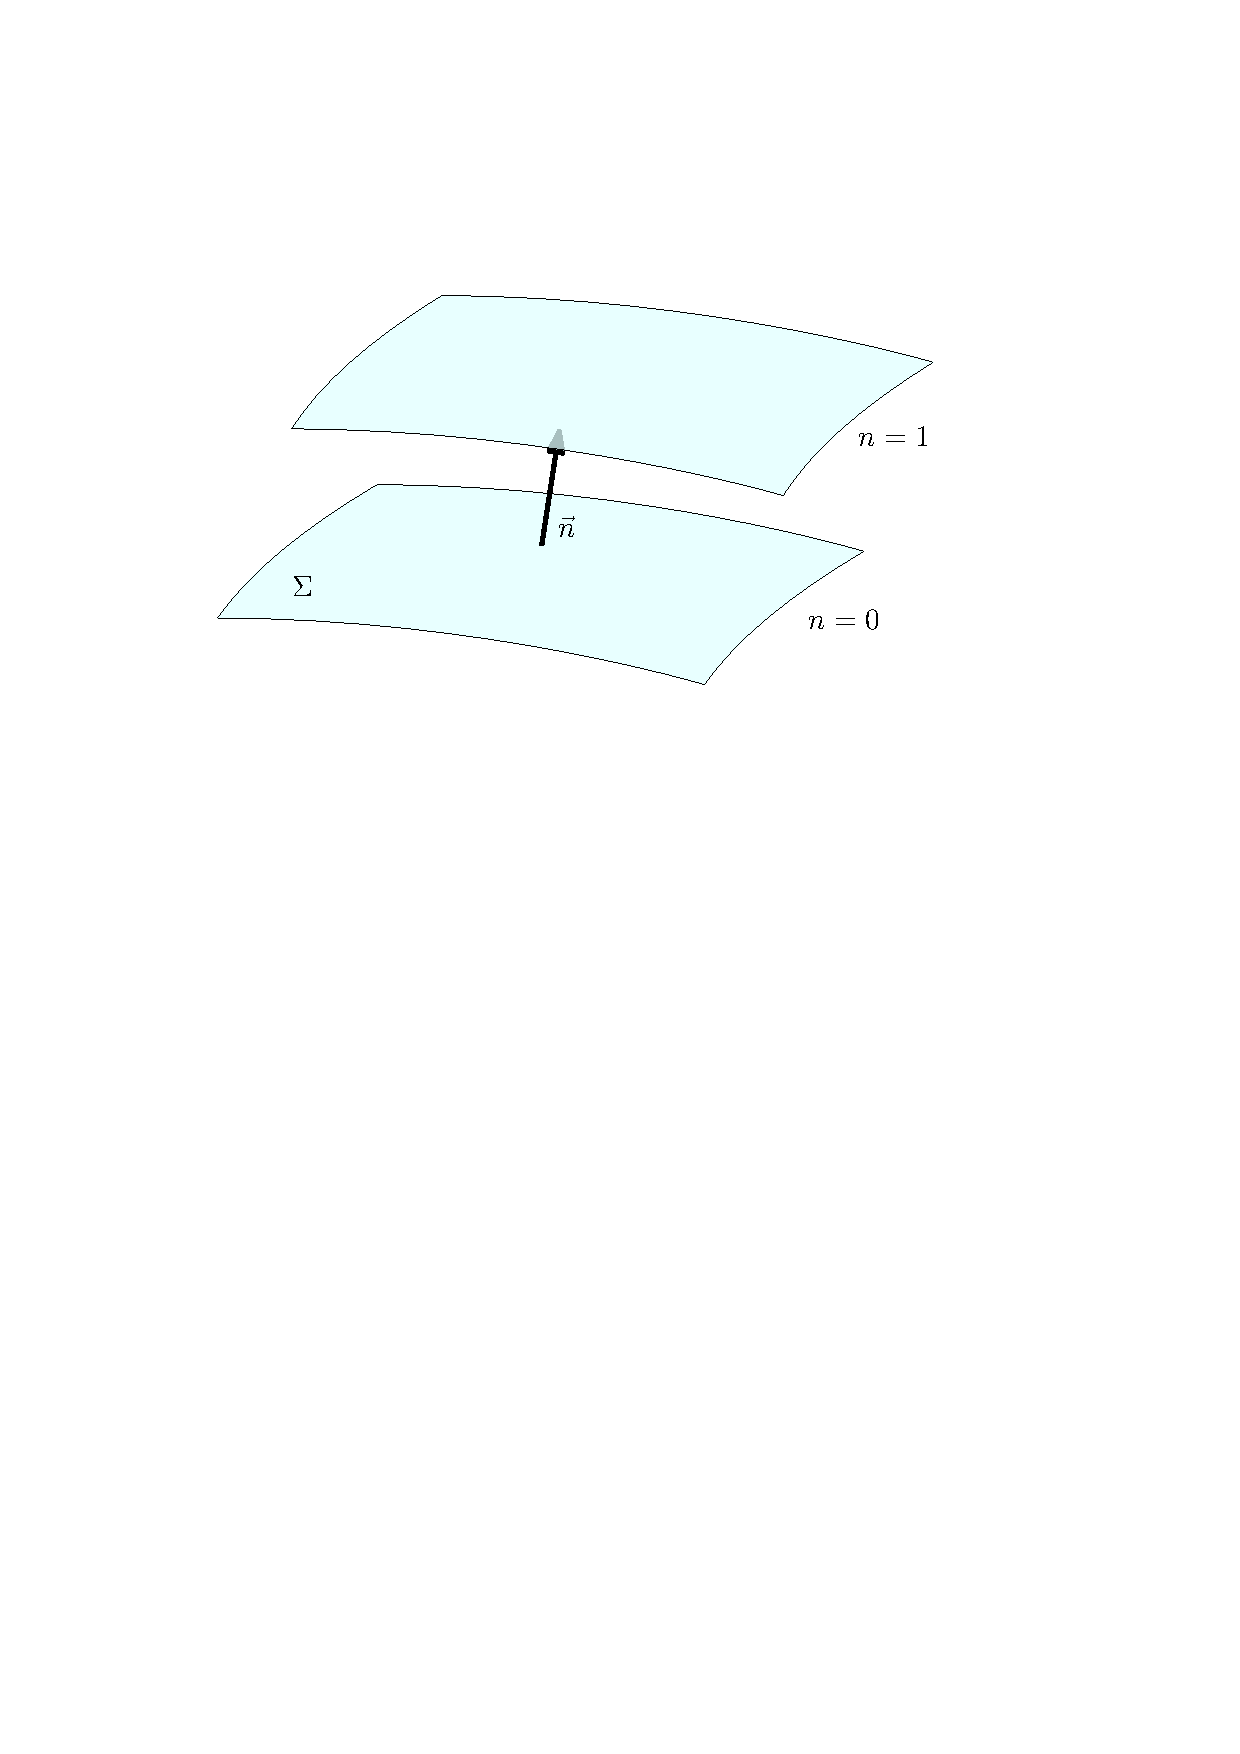
\includegraphics[width=0.7\linewidth]{figures/Junction.pdf}
     \caption{Coordenadas Gausianas en el vecindario a $\Sigma$}
     \label{JC}
 \end{figure}
Las condiciones de acoplamiento en este "set-up" son:
 \begin{enumerate}[leftmargin=2cm]
     \item La métrica inducida $g_{ij}$ es continua a través de $\Sigma$.
     \item El tensor de energía-momento superficial se anula en la superficie
     \begin{equation}
\lim _{\varepsilon \rightarrow 0}\left[\int_{-e}^{+\varepsilon} T_{\beta}^{\alpha} d n\right]=0.
    \end{equation}
     
 \end{enumerate}
 
 \textbf{C2:} Para el caso considerado en este trabajo $\Sigma:\,r=R$, además la simetría esférica permite identificar $\vec{n}=\pdv{r}$ y debido a que la solución externa es de vacío $\eval{T^{\alpha}_{\beta}}_{+\epsilon}$= 0, bajo estas condiciones las condiciones de acoplamiento se reducen a
 \begin{enumerate}[leftmargin=2cm]
     \item $e ^ {  2 \nu(R) } =  1 - \frac { 2 M } { R }$.
    \item $P(R)=\rho(R)=0$.
 \end{enumerate}


\subsection*{ Sobre el corrimiento al rojo gravitacional}
La luz emitida por una estrella es observada corrida al rojo por un observador lejano debido a la presencia del campo gravitacional. Qué tanto es corrida al rojo puede ser estimado de manera sencilla \cite{Glendenning2000}: considerando un átomo de la estrella a una distancia $r$ de su centro, que emite un fotones con determinada frecuencia, el intervalo de tiempo propio entre dos emisiones consecutivas está dado por
\begin{equation}
d \tau=\sqrt{-g_{\mu \nu} d x^{\mu} d x^{\nu}},
\end{equation}
en el marco del átomo esto es simplemente ($dx^i=0$)
\begin{equation}
d \tau_{\mathrm{e}}=\sqrt{-g_{00}(r)} d t.
\end{equation}
Si suponemos que el observador y el átomo yacen sobre la misma línea el intervalo espacio-temporal para la radiación es
\begin{equation}
d \tau^{2}=g_{11}(r) d r^{2} - g_{00}(r) d t^{2} = 0,
\end{equation}
así que el tiempo que tardó un ciclo en viajar de $r$ a $\infty$ es
\begin{equation}
\Delta t=t_{\infty}-t_{R}=\int_{R}^{\infty}\left(\frac{g_{11}(r)}{g_{00}(r)}\right)^{1 / 2} d r,
\end{equation}
es decir, $dt$ (tiempo coordenado entre dos emisiones consecutivas) es el mismo para el emisor y el observador lejano. Con lo anterior, el tiempo propio para el observador será
\begin{equation}
d \tau_{\mathrm{o}}=\sqrt{-g_{00}(\infty)} d t.
\end{equation}
Como el inverso del tiempo propio es proporcional a la frecuencia, la razón entre la frecuencia emitida y observada es
\begin{equation}
\frac{\omega_{\mathrm{e}}}{\omega_{\mathrm{0}}}=\left(\frac{g_{00}(\infty)}{g_{00}(r)}\right)^{1 / 2}=e^{-\nu(r)},
\end{equation}
y con esto el corrimiento al rojo gravitacional es
\begin{equation}
    z(r)\equiv \frac{\omega_{\mathrm{e}}-\omega_{\mathrm{o}}}{\omega_{\mathrm{o}}}  = e^{-\nu(r)}-1.
    \label{redshift}
\end{equation}
\textbf{C3:} El corrimiento al rojo descrito por \eqref{redshift} debe disminuir con el incremento de $r$.
\subsection*{Sobre el signo de la densidad de energía y la presión}
La densidad de energía y la presión deben ser positivas dentro de la estrella.\TODO{Materia normal?}

\subsection*{Sobre la densidad de energía y la presión}
\textbf{C5:} La densidad de energía y la presión deben alcanzar un máximo en el centro ($\rho'(0)=P'(0)=0$) y deben decrecer monótonamente hacia afuera.\TODO{Decrecimiento monótono?}

\subsection*{Condiciones de energía}
Con el fin de obtener soluciones a las ecuaciones de Einstein en presencia de fuentes de energía y momento realistas es necesario imponer ciertas condiciones de energía que limiten la arbitrariedad del tensor energía-momentum escogido.

Existe una variedad de condiciones de energía que son usadas en diferentes circunstancias, las usadas con mayor frecuencia son \cite{Hawking1973TheSpaceTime,Carroll2003SpacetimeRelativity}:

\begin{itemize}[leftmargin=1.5cm]
    \item \emph{Condición de energía débil}: el tensor de energía-momentum en cada punto $p$ de la variedad obedece la desigualdad $T_{\mu \nu} t^{\mu} t^{\nu} \geq 0$ para cualquier vector tipo tiempo $t^{\mu}\in T_{p}$.
    \item \emph{Condición de energía dominante}: el tensor de energía-momentum en cada punto $p$ de la variedad obedece la desigualdad $T_{\mu \nu} t^{\mu} t^{\nu} \geq 0$ y además $T^{\mu \nu} t_{\mu}$ es un vector que no es tipo espacio para cualquier vector tipo tiempo $t^{\mu}\in T_{p}$.
    \item \emph{Condición de energía fuerte}: el tensor de energía-momentum en cada punto $p$ de la variedad obedece la desigualdad $T_{\mu \nu} t^{\mu} t^{\nu} \geq \frac{1}{2} T_{\lambda}^{\lambda} t^{\sigma} t_{\sigma}$, para cualquier vector tipo tiempo $t^{\mu}\in T_{p}$.
\end{itemize}
Mientras que las condiciones débil y fuerte no se cumplen para el tensor energía-momento de algunos campos escalares con $m=0$ y $m\neq 0$ respectivamente \cite{Hawking1973TheSpaceTime}, la dominante es cumplida por todas las formas de materia conocidas y se requerirá por lo tanto que la materia en las estrellas de neutrones la cumpla. 

Escribiendo $t^\nu$ en una tétrada ortonormal $e_{\mu}$ como
\begin{equation}
    t^{\mu} e_{\mu}= \left(1+a^{2}+b^{2}+c^{2}\right)^{1 / 2} e_{0}+a e_{1}+b e_{2}+c e_{3},
\end{equation}
con el tensor de energía-momento de un fluido perfecto que se está considerando \eqref{EMT}, la condición $T_{\mu \nu} t^{\mu} t^{\nu} \geq 0$ se puede escribir como
\begin{equation}
T_{\mu \nu} v^{\mu} v^{\nu}=\left(1+a^{2}+b^{2}+c^{2}\right) \rho + \left( a^{2} +b^{2} +c^{2} \right) P \geq 0 \quad \forall a,b,c \in \mathbb{R},
\end{equation}
para el caso $a=b=c=0$ esto implica $\rho \geq 0$ y en el límite en que $a^2+b^2+c^2 \to \infty$ que $\rho + P \geq 0$.

Además, con $T^{\mu \nu} t_{\mu}$ escrito como
\begin{equation}
T^{\mu \nu} t_{\mu}e_{\nu}=\left(1+a^{2}+b^{2}+c^{2}\right)^{1 / 2} \rho e_{0}+a P e_{1}+b P e_{2}+c P e_{3},
\end{equation}
la condición de que no sea tipo espacio se convierte en
\begin{equation}
    -\rho^2 + (P^2-\rho^2)(a^2+b^2+c^2) \leq 0 \quad \forall a,b,c \in \mathbb{R},
\end{equation}
lo cual implica que $\rho \geq |P|$.

Debido a que en C1 se requirió que $\rho$ y $P$ fueran positivas, la condición de energía dominante añade la restricción $\rho \geq P$.

\textbf{C6:} La solución debe satisfacer la condición $\rho \geq P$.

\subsection*{Condición de causalidad}
El postulado de causalidad local en relatividad general prohíbe que alguna señal se propague a una velocidad mayor que la velocidad de la luz \cite{Hawking1973TheSpaceTime}. 

\textbf{C7:}  La velocidad del sonido en la estrella (modelada como un fluido) está dada por []\TODO{Usar una cita de algún libro de hidrodinámica}
\begin{equation}
    v^2=\dv{P}{\rho},
\end{equation}
y esta no puede sobrepasar la velocidad de la luz:
\begin{equation}
    0 < \dv{P}{\rho} \leq 1 .
\end{equation}
\REMARK{La presión y densidad son cantidades definidas localmente, así que la velocidad del sonido local debe ser menor a la velocidad de la luz.}

\subsection*{Criterio de estabilidad del índice adiabático }
\REMARK{$\Gamma=4/3$ para un gas polítropo relativista, pero este valor puede variar a lo largo de la estrella y ser menor. Las condiciones de estabilidad están dadas para el índice adiabático efectivo. Revisar con el profesor.}

\textbf{C8:} El índice adiabático debe satisfacer
\begin{equation}
    \Gamma = \frac { \rho + P  } { P } \dv{P}{\rho} \geq \frac{4}{3}.
\end{equation}

\subsection*{Estabilidad ante cracking}
El cracking es una posible inestabilidad de esferas autogravitantes ante perturbaciones locales.

\textbf{C9:} El criterio para que una distribución sea estable ante cracking presentada por Nuñez et al. \cite{Gonzalez2014CrackingSpheres} es
\begin{equation}
    0 \geq \dv{P}{r}.
\end{equation}

\subsection*{Estabilidad ante pulsaciones radiales. Criterio de Harrison-Zeldovich-Novikov}
Cuando se considera la estabilidad global de una configuraci\'on de energía con simetría esférica, se analiza cómo pulsaciones radiales pueden inducir el cuerpo a colapsar. 

\textbf{C10:} La estabilidad en este método estará determinada por la frecuencia del modo fundamental de oscilación (ver \cite{Haensel2007NeutronStructure,Shapiro1983}), sin embargo una condición más práctica para determinar si una configuraci\'on con simetría esférica es inestable globalmente es la conocida condición de Harrison-Zeldovich-Novikov, la cual enuncia que para una configuración sea estable respecto a oscilaciones radiales es \emph{necesario} que su masa $M$ aumente a medida que la densidad central $\rho_{c}$ crece: 

\begin{equation}
    \frac { \partial M \left( \rho _ { c } \right) } { \partial \rho _ { c } } > 0.
\end{equation}
Además, los puntos en los que $\frac { \partial M \left( \rho _ { c } \right) } { \partial \rho _ { c } } = 0$ (puntos críticos) son puntos donde la configuraci\'on pasa de estabilidad a inestabilidad.



\subsection*{Estabilidad ante convección adiabática}

La estabilidad contra convección se puede entender como sigue: cuando un elemento de fluido es desplazado hacia abajo, si su densidad aumenta más rápido que la densidad que lo rodea, el elemento se hundirá y la configuraci\'on será inestable. Por otro lado, si la densidad del elemento de fluido es menor que la de su alrededor, flotará y la estrella será estable contra convección.

\textbf{C11:} En el caso en que la perturbación del elemento de fluido es adiabática (pasa en intervalos de tiempo muy pequeños comparados con los del flujo de calor) Nuñez et al. \cite{Hernandez2018} mostraron que para que el modelo estelar fuera estable contra movimientos convectivos, el perfil de densidad $\rho(r)$ debe cumplir el siguiente criterio: 
\begin{equation}
    \rho ^ { \prime \prime } ( r ) \leq 0.
\end{equation}